\chapter{Design}
Now we know exactly what we want our project to do, so it is time to design \emph{how} we are going to do it. We already defined the
architecture which will point the path to follow, and divide the design efforts in four parts: main daemon, command line daemon controller,
library and the plugins interface.
\section{Daemon}
% TODO Extend report contents
Called \emph{reactord} is the central program of the project.
\begin{list}{-}{It mainly has to:}
  \item Locate the rules files.
  \item Parse the rules files.
  \item Receive control commands.
  \item Receive remote events.
  \item Register and run the plugins.
  \item Manage the state machines.
%   \item Notice the events.
%   \item Trigger the actions.
\end{list}
Before we start discussing these points in deep we will explain the users restrictions to use this daemon. We have to say these 
restrictions are not entirely implemented for the final project for lack of time, but they were kept in mind in order to easily satisfy 
them in a near future.
\subsection{User restrictions}
\label{sec:users}
As you probably already know, UNIX is a multi-user system in which there is the \emph{root} user, also known as \emph{superuser}, who has 
permissions to access all the files, and then there are the other users, which could have more restrictive permissions. These users can
be organized in groups so we can set permissions to a whole set of concrete users to restrict them to certain files.\\
We will make use of this and divide the potential users of \emph{reactor} in three sets with different access to the main daemon. These
groups will be \emph{administrators}, \emph{reactor group users} and \emph{others}. The goal of this division is to give daemon access 
to the major numbers of users in a system while isolating some security issues and keeping it as a one instance only program.\\
\emph{Administrators} is in fact just the \emph{root} user, but we name it in plural because we are considering all the users with access 
to \emph{root} user, either by \emph{sudoers} file\footnote{\emph{sudoers} is a file which defines the users that can execute commands as 
superuser by using the \texttt{sudo} command.} or \emph{wheel} group\footnote{The \emph{wheel} group is an inheritance of UNIX. It is a 
group that contains the users with access to \texttt{su} command.}. But the final user is always one, \emph{root}.\\
By \emph{reactor group users} we understand all the users that the system administrators choose to have some privileges that we will see 
in the following lines. They are all in a predefined user group, by default called \emph{events}.\\
\emph{Others} are simply the other users not considered by the two previous groups. Their access to \emph{reactord} is not controlled by 
the system administrators so, for security reasons, this must be the most restricted group.\\
\begin{table}[h]
  \begin{subtable}[h]{1\textwidth}
    \centering
    \begin{tabular}{p{2.5cm}|c|c|c|}
      \cline{2-4}
      & \multicolumn{3}{|c|}{Users} \\ \cline{2-4}
      & Administrators & \emph{reactor} group users & Others  \\ \cline{1-4}
      \multicolumn{1}{|p{2.5cm}|} {Start \emph{reactord}} & \Checkmark & \XSolidBrush & \XSolidBrush \\ \cline{1-4}
      \multicolumn{1}{|p{2.5cm}|} {Rules file} & \texttt{/etc/reactor.d/reactor.rules} & \texttt{\~{}/.reactor.rules} & \XSolidBrush \\ \cline{1-4}
      \multicolumn{1}{|p{2.5cm}|} {Actions user} & \emph{root} & User & User \\ \cline{1-4}
      \multicolumn{1}{|p{2.5cm}|} {Plugins events notice} & \Checkmark & \Checkmark & \Checkmark \\ \cline{1-4}
    \end{tabular}
    \subcaption{General restrictions}
  \end{subtable}
\\
\\
\\
  \begin{subtable}[h]{1\textwidth}
    \centering
    \begin{tabular}{p{1.5cm}c|c|c|c|}
      \cline{3-5}
      & & \multicolumn{3}{|c|}{\emph{libreactor} messages send by} \\ \cline{3-5}
      & & Administrators & \emph{reactor} group users & Others \\ \cline{1-5}
      \multicolumn{1}{|p{1.5cm}|}{\multirow{3}{1.5cm}{Valid SMs owners}} & \multicolumn{1}{|c|}{Administrators} & \Checkmark & \XSolidBrush & \XSolidBrush \\ \cline{2-5}
      \multicolumn{1}{|c|}{} & \multicolumn{1}{|c|}{\emph{reactor} group users} & \Checkmark & \Checkmark\tiny{If same user} & \XSolidBrush \\ \cline{2-5}
      \multicolumn{1}{|c|}{} & \multicolumn{1}{|c|}{Others} & \Checkmark & \Checkmark & \Checkmark\tiny{If same user} \\ \cline{1-5}
    \end{tabular}
    \subcaption{Valid \emph{libreactor} messages by user senders and owners of the receiving state machines.}
    \label{tab:restlib}
  \end{subtable}
  \caption{Summary of the \emph{reactor} user restrictions}
  \label{tab:rest}
\end{table}
In \emph{tables \ref{tab:rest}} we can see a summary of the restrictions for every kind of user. As we can see, \emph{root} is the only
user that can start the daemon. Also remember that \emph{reactord} must check that there is not another instance running before it starts.
This is a very common behaviour in UNIX systems.\\
The principal difference between the three sets of users is the location of the rule files, which every user has a different one. For the 
administrators state machines we have an standard location for \emph{root} configuration files (\texttt{/etc/reactor.d/reactor.rules}).
This file, and all the files in the same directory, will be readable by all the users but only writeable by the system administrators.
The rule files for the \emph{reactor} group users will be located in theirs \emph{home} directory (\texttt{\~{}}), and hidden (therefore 
the '.' prefix) so it does not bother the user by showing with his documents. Others do not have rule files so they can not have state 
machines running every time the operating system boots. In the other hand they can load state machines with \emph{reactorctl} manually or 
using a session initialization script, in order to automatically load the rules every time the user logs in. May be it would be interesting
for the system administrators that when these other users log out, their states machines would be automatically unloaded. A solution is 
described on section \ref{sec:future}.\\
Some kinds of actions of the state machines we have may need an \emph{uid}\footnote{Stands for 'user identifier'. Is the number used in 
UNIX-like operating systems to identify a user.} to be performed. By now this is only the command actions, which needs an \emph{uid} to 
make it the user owner of the process, and so restrict it to access the filesystem. Superuser obviously does not need any restriction on
its state machine actions (actually it doesn't make sense). But the rest of the users must run their state machines and execute its 
actions as their own, so we do not put the integrity of the operating system in danger. Also we must not allow a state machine to have
a transition to another user's state machine for the same reason.\\
There is one last thing to control about the users. Users can send control messages to the \emph{reactord} through programs using the 
\emph{libreactor} shared library, or the \emph{reactorctl} program that, as it is explained later, is actually using \emph{libreactor}. 
Therefore, for example, the \emph{others} set of users may send an event that makes malfunction a \emph{root}'s state machine, or simply 
delete all its state machines. To avoid this we should set credentials to the events send by \emph{libreactor}. And that is what we can see
at \emph{table \ref{tab:restlib}}. Administrators state machines can only rely on their own control messages and not on the rest of the 
users'. 'events' state machines will work with both their own users' control messages and \emph{root}'s, and finally \emph{others} can rely
on all the control messages, except for the other users without higher credentials. Notice a user can not send control messages in order 
to change or forward another user's state machine from the same set of users. But what about remote events? If there is no control for the 
remote events as well, the same \emph{others} user may propagate an event to another device, or even to localhost, 
that makes it execute an unintended \emph{root} command. This problem is trickier than the \emph{libreactor}'s, because the connection
only gives us the address of the remote \emph{reactord} but neither the user, nor even the source program. A simple event message could be
sent with a tool like \texttt{telnet} easily. To solve this we set several configurable security levels:
\begin{enumerate}
 \item Leave all the plain events in.
 \item Set the address which we expect events to arrive from.
 \item Encrypt event messages with TLS.
 \item Mutual authentication using TLS.
\end{enumerate}
This solution is the same that they use in \emph{syslog-ng}\cite{man:syslog-ng} for receiving remote log messages, and probably in many 
more projects.
\subsection{Rule parsing}
% TODO Definir les regles de crontab amb el nostre pre-parser.
\label{sec:rparser}
At the beginning of the section we made a list of the internal functionalities in which we can divide \emph{reactord}, and we will follow 
them more or less to explain its design. The location of the rule files is explained in the previous subsection, we have a unique file for 
the administrators, and we have to check which are the members of the 'events' group in order to read the file from their 'home' 
directories. This is one of the first things the daemon has to do.\\
The next thing is to get and to process the information from those files, and parse them. At the beginning of the development the whole 
parser was a component of \emph{reactord} but, when developing the plugins part, it became necessary to share it in \emph{libreactor}, 
so it could be used for the plugins as well, or at least a part of it.\\
There are some properties that the rules from a plugin and from the daemon are more likely to share. For example a rule, that in our case
is the minimal unit to define complete information about how we want our system to behave, will be one line only. Also, in general
and as an implication one-line/one-rule property, those rules won't have a complex syntax. This syntax can be defined similarly to a markup
language. We can define an expressions in a line by subexpression separator and expression end tokens. The next line is a valid 
\emph{reactor} rule:
\begin{center}
  \texttt{state\_a state\_b event1 \&event2\&event3 \& event4 \&event5 PROP myserver:6500\\}
\end{center}
The two tokens from the beginning, \texttt{state\_a} and \texttt{state\_b}, are the out state and the in state of the transition we are
defining. From the next token until \texttt{PROP} we have the list of events to notice before we forward to the in state, separated by the
\texttt{\&} character. At least one event is required. From \texttt{PROP} until the end of the line is the action to perform. \texttt{PROP}
is the kind of the action, in this case it is a propagation action. We have three different kinds of actions:
\begin{itemize}
  \item \texttt{NONE}\\
    Do not perform any action. It is not followed by any action definition.
  \item \texttt{CMD}\\
    Run a command in a shell. It is followed by the command itself.\\
    i.e.:  \texttt{CMD echo ``OK > /tmp/test}
  \item \texttt{PROP}\\
    Propagate all the events from the rule to an IP address. It is followed by the address with the format \emph{host:port}, or \emph{host}
    for the default \emph{reactor} port.\\
    i.e.: \texttt{PROP publicserver.com}
\end{itemize}
So the simplified syntax would be:\\
\begin{center}
  leaving\_state destination\_state list \& of \& events TYPE\_OF\_ACTION action
\end{center}
In \emph{figure \ref{fig:rulesm}} we have the resulting state machine from the example rule.\\
\begin{figure}[t]
  \centering
  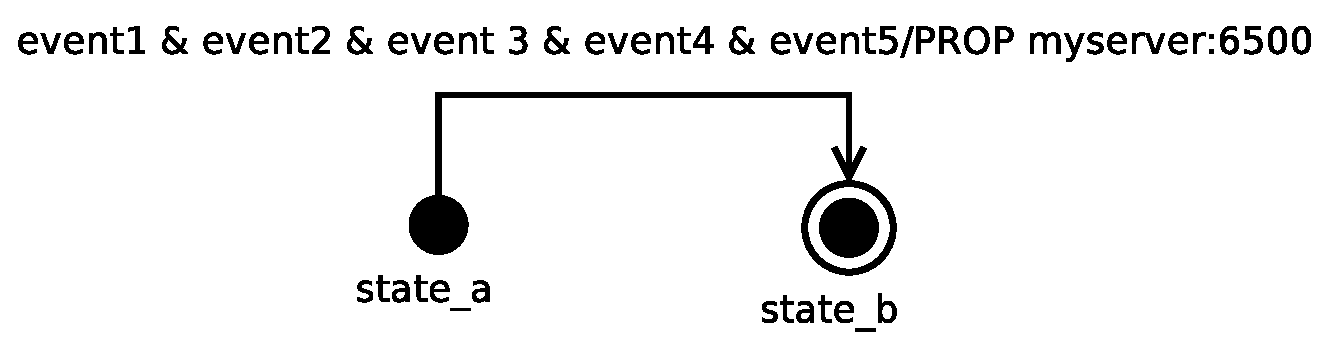
\includegraphics[width=0.8\textwidth,keepaspectratio]{img/rulesm}
  \caption{Resulting state machine from the example rule.}
  \label{fig:rulesm}
\end{figure}
With the simple kind of grammars we previously explained we can tokenize the rule and build an initial parse tree. The main expression
has separated tokens with the space character, and with a \texttt{End-Of-Line} terminal character. The third token is the beginning of a 
subexpression tokens separated by the \texttt{\&} character and with the space character as terminal. Finally, the fourth token (we are
counting the subexpressions as a single tokens) has \texttt{End-Of-Line} as terminal character and the same as separator (it has no 
separators). With this grammar we get the parse tree in \emph{figure \ref{fig:initparsetree}}.
\begin{figure}[t]
  \centering
  \includegraphics[width=.65\textwidth,keepaspectratio]{img/initparsetree}
  \caption{Resulting parse tree from the example rule with the explained grammar.}
  \label{fig:initparsetree}
\end{figure}
As we know how the syntax of the plugins rules may look like (the subset of grammars), but not how exactly how they will be, we made a 
generic simple parser in which you specify the parameters explained before and we get a parse tree like the one in \emph{figure 
\ref{fig:initparsetree}}. But this one is not exactly the parse tree \emph{reactord} needs. The 'action' branch gives the 'PROP' unparsed,
and it needs the kind of action, the host and the port separated in different nodes. This can't be done with our initial parsing function
because we do not support conditional subexpressions. That is we can not expect a subexpression after \texttt{PROP}, but a different
one after \texttt{NONE} or \texttt{CMD}. We need the final part of the parsing process to be done in \emph{reactord}. The process well be
limited to receive the unfinished parse tree, go to the target branch (fourth from root) and parse it with the action kinds conditions.
If its \texttt{NONE} there can't be nothing after it, so the action node will have only a leaf child with the content ``NONE''. If we 
have a \texttt{CMD} action it has to make a node with the content ``CMD'' and a single leaf child with the command in it. In the case of 
our example we expect two leaf children in the ``PROP'' node, one with the host and the other one with the port, as shown in \emph{figure
\ref{fig:finalparsetree}}.
\begin{figure}[t]
  \centering
  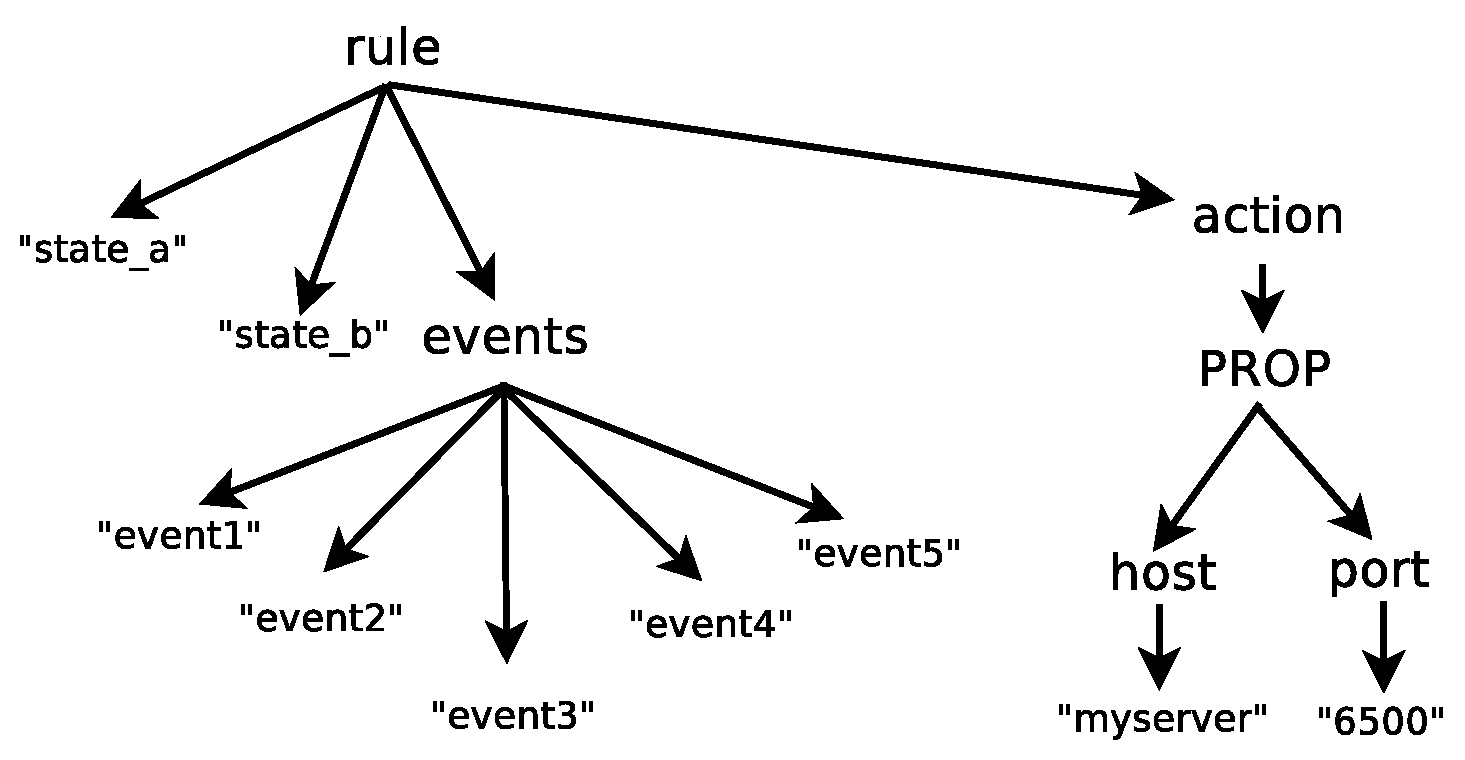
\includegraphics[width=.8\textwidth,keepaspectratio]{img/finalparsetree}
  \caption{Resulting parse tree from final parse process in \emph{reactord}.}
  \label{fig:finalparsetree}
\end{figure}
The parse tree also contain information about the line number and file of every rule, and informs about errors. This will be explained in
detail in the plugin's \emph{section \ref{sec:parser}}.\\ 
Now the parse tree is ready to be sent to a function which adds the actual transition to our states machines.
% TODO Speak about errors.
\subsection{Control messages handling}
As with the parser, the great part of code of the \emph{reactord} control communication was moved to \emph{libreactor} during the 
development.
This is the code in charge of communicating \emph{reactorctl} and other programs running in the same operating system with \emph{reactord}.
Once \emph{reactord} has been initialized, it is permanently waiting for control messages. The format of a message will be detailed
in \emph{section \ref{sec:cntrl}} as the it is defined in \emph{libreactor} as well, but by now we can consider that it has an 
identifier of the message type and the message data. Therefore when a message is sent to \emph{reactord}, it is processed by a callback 
function. This function checks the message expecting three kinds of message and act consequently:
\begin{itemize}
% TODO Make an error for credentials mismatch?
  \item \texttt{EVENT}\\
    The data fields of the message are an event identifier and the credentials of the sender. This information is sent to the event handling
    function at once. The sender program expects an \texttt{ACK} message in return.
  \item \texttt{ADD\_RULE}\\
    It comes with a rule in exactly the same form as in the rule files and the credentials of the sender. It is sent to the parser as a 
    single rule instead of a whole file like in the previous section. The parse tree is sent to the transition adding function. The sender 
    expects a response. If everything went fine it will receive an \texttt{ACK}, but if the rule was malformed or another error happened, 
    it will receive \texttt{ARG\_MALFORMED}. Errors will be logged using \emph{libreactor}.
  \item \texttt{RM\_TRANS}\\
    Contains an state identifier, a number to identify a leaving transition and the credentials of the sender. It is intended that in
    the future we have a way to visualize the state machines as graphs in which every transition has a number identifying it using 
    graphviz\cite{graphviz} or/and similar tools. This number will simply be the order in which the transition was inserted 
    (\emph{section \ref{sec:future}}). The data will be sent to the transition removing function. In case everything went well the sender 
    must receive \texttt{ACK}, but \texttt{ARG\_MALFORMED} otherwise. Errors will be logged using \emph{libreactor}.
\end{itemize}
\subsection{Remote events handling}
The remote events handling uses the same tools from \emph{libreactor} than the local control messaging system, but over the TCP/IP 
protocol.\\
Before the remote sender begins to send events to the local \emph{reactord} a plain connection negotiation is needed. The local and the
remote hosts need to compare their versions of the software so they can decide which connection-related features are available and
so if the connection can be performed. Then the local host will inform about the conditions of the connection to the remote client, which 
can be accepted or rejected. Those conditions are extracted from a configuration file. When the conditions are accepted then connection
begins. If the configuration states that the connection must be authenticated TLS, we should have the remote certificate linked to
a local user in order to assign credentials.\\
Like with the \texttt{EVENT} case, the sender expects an ACK after every event received. The difference with the local control messages is
that the connection keeps open until the sender has sent all the events. The sender will inform about the end of the set of events with an
\texttt{EOM}\footnote{EOM stands for End Of Message} message. If the \texttt{EOM} is not received, it can be considered an error.\\
\subsection{Plugins management}
\begin{list}{-}{The \emph{reactor} plugin system is formed by four parts:}
  \item Plugin API.
  \item Plugin interface.
  \item Plugin manager.
  \item The plugins.
\end{list}
The {\bf plugin API} is the set of functions available from \emph{libreactor} and the callbacks sent by \emph{reactord}. The main functionality
from \emph{libreactor} expected to be used in the plugins is the generic parser explained in \emph{\ref{sec:parser}}, and logging 
functions (\emph{section\ref{sec:log}}). The 
\emph{reactord} callbacks are the functions from the daemon that  it set available for the plugin in the registration process. By now
the only callback the plugin can expect is the event handling function, so it can make \emph{reactord} notice events directly.\\
The {\bf plugin interface} is also in \emph{libreactor} and is the specification of the expected functions that the plugin has to implement.
It also contains the data structures definitions shared by \emph{reactord} and the plugins. Explained in \emph{section 
\ref{sec:plugins}}.\\
The {\bf plugin manager} is the piece of code of \emph{reactord} that is in charge of the communication with the plugin interface. It loads the
plugins from the directory where they are supposed to be located, initializes them and sets them into a list. When we want to unload a
plugin it is done by the plugin manager too. By now this is the only things it does, but when poll-like information is needed from the 
plugins, it will manage the plugins and the functions to call.\\
The {\bf plugins} are implementations of the different functions from the interface. Explained in \emph{section \ref{sec:plugins}}.\\
In \emph{figure \ref{fig:pluginsdia}} we can see the generic behaviour of the plugins system.
\begin{figure}[h]
  \centering
  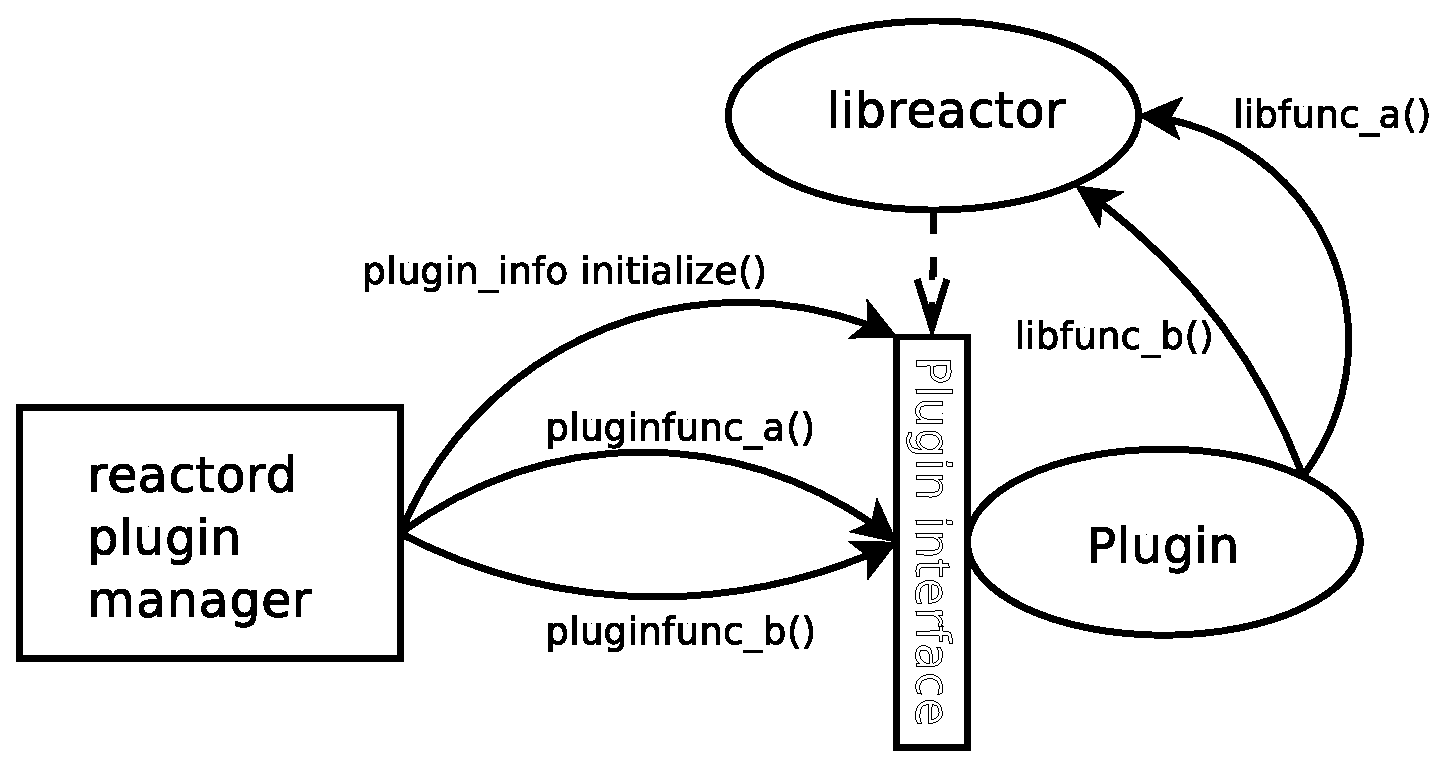
\includegraphics[width=0.8\textwidth,keepaspectratio]{img/pluginsdia}
  \caption{Generic behaviour of the \emph{reactord} event system.}
  \label{fig:pluginsdia}
\end{figure}
The return variable from the \texttt{initialize()} function is a set of plugin information values and callbacks to the plugins functions.
In our case, the plugins are only launched as workers. This means that we will call a plugin main function as a thread which will be 
running until we stop it, or until we stop \emph{reactord}. This function is expected to be the main function for the new events 
sensors, and it should call the \emph{reactord} event handling function every time an expected event is detected. Of course by the 
initialization phase we are talking about the parse of the plugin's rules file.\\
So, the functions called after the \texttt{initialize()} function are those callbacks returned by the plugin, and in our case is the 
worker's main function.\\
The \emph{libfunc\_x()} functions is where the parser call would be.

\subsection{State machine management}
\label{sec:smman}
We have now management actions over the state machines ready to be performed. In order to perform them, we have three input handlers 
functions:
\begin{itemize}
  \item Add-transition handler.
  \item Remove-transition handler.
  \item Event handler
\end{itemize}
The {\bf add-transition} handler is a function that expects the parse tree of a rule and the credentials of its owner. It starts by checking 
for errors in the parse tree. Remember that when the parser founds a syntax error in a rule, it writes the error on the parse tree. If 
there are any it will stop and return an error value. It checks next if the states of
the transition already exists and in which state machines they are. If the states are in different state machines (and this includes an
initial leaving state going to an existing non-initial state) the addition of the transition becomes illegal. We log the error and return 
an error code. The reason for this is that the state machines become a state machine with several initial states. In \emph{reactor} an 
initial state is an execution of the state machine. If we have several initial states then we have several executions of the same state
machine, and this makes the design a lot more complex. This is illustrated in \emph{figure \ref{fig:illegalsm1}}.\\
\begin{figure}[b]
  \centering
  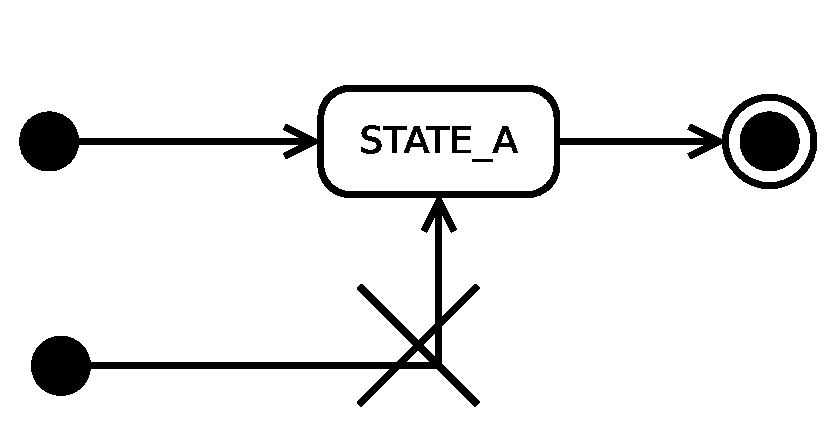
\includegraphics[width=0.5\textwidth,keepaspectratio]{img/illegalsm1}
  \caption{Illegal transition addition from an initial state to an existing non-initial state.}
  \label{fig:illegalsm1}
\end{figure}
Another illegal addition to check is the case in which the user is trying to add to connect two states machines of different users.
You may understood that every transition connecting different states machines are illegal. But the case in which we are connecting an state
to the initial state of another state machine is legal, because the result is an state machine with just one initial state. The problem 
comes when the user is trying to connect an state machine of his own with another of higher credentials, because he would be able to leave
the other user's state machine unable to start by for example setting a new initial transition with an nonexistent event for its activation.
We see it illustrated in \emph{figure \ref{fig:illegalintersm}}. In \emph{figure \ref{fig:intersm}} we can see that the transition
addition becomes legal by simply reverting the user roles.
\begin{figure}[h]
  \centering
  \begin{subfigure}[b]{0.45\textwidth}
    \centering
    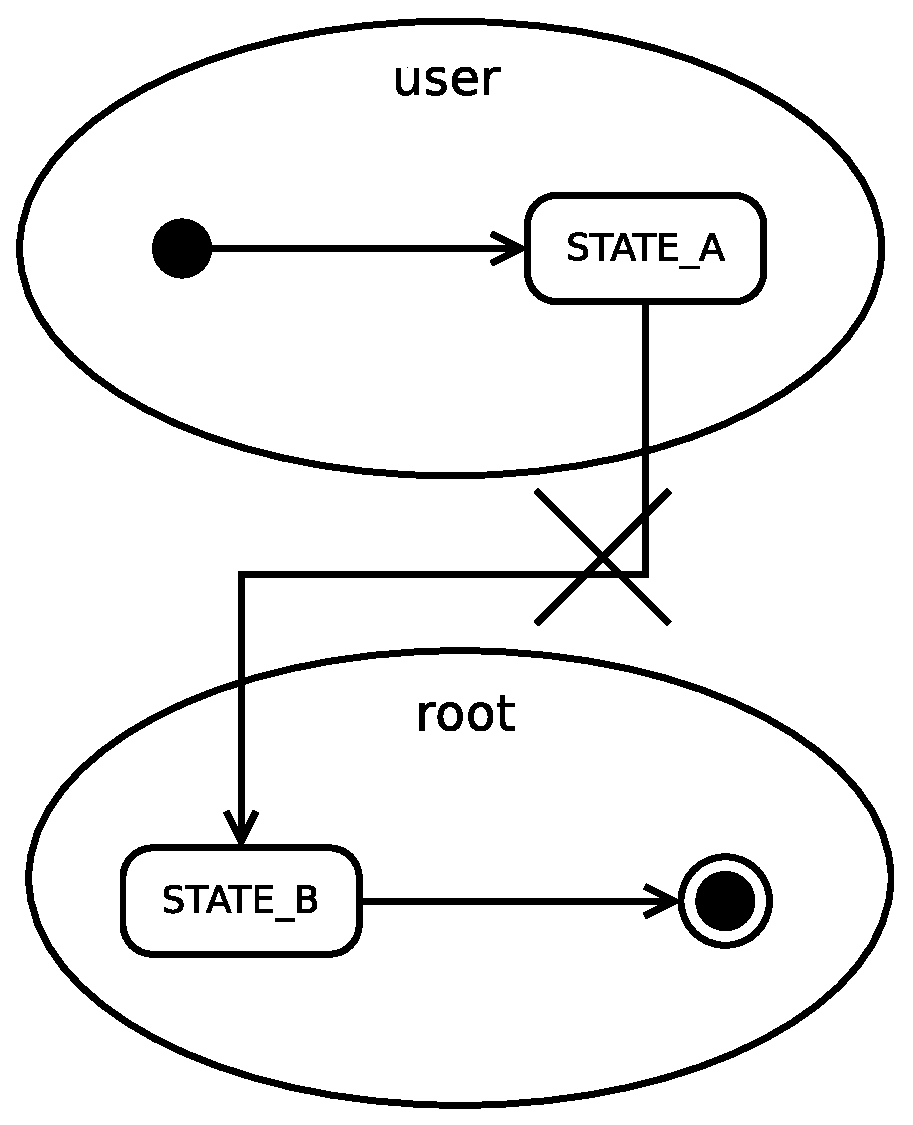
\includegraphics[width=\textwidth,keepaspectratio]{img/illegalintersm}
    \caption{Illegal transition addition from a lower credential user state machine to a higher credential user state machine.}
    \label{fig:illegalintersm}
  \end{subfigure}
  ~
  \begin{subfigure}[b]{0.45\textwidth}
    \centering
    \includegraphics[width=\textwidth,keepaspectratio]{img/intersm}
    \caption{Legal transition addition from a higher credential user state machine to a lower credential user state machine.}
    \label{fig:intersm}
  \end{subfigure}
  \caption{State machine inter-user connection example.}
\end{figure}
Once these checks are passed without problem we save the new states and link them with a transition. We also locate the events in a hash
table in order to access them later when we receive their event identifiers. If the transition can be forwarded immediately (the leaving 
state is initial or is the current state of the state machine) then the transition is set in a current transitions list on the its events.
This way the transitions are easily accessible every time we notice an event as well.\\
\\
The {\bf remove-transition handler} needs a leaving state identifier with a number identifying one of its leaving transitions and the user 
credentials. It has to perform two checks. The first one is the credentials check, it means that a lower privileged user can't remove a 
transition from a higher privileged user. The other check is the existence of the transition. In both cases, if the checks fail, it will
stop and return an error value.\\
Now it is good to remove the transition. To do so it unlinks the leaving state from the transition and the transition from the entry state.
So we are removing a reference from the entry state. When we remove all the references from an state we remove this state as well, removing
all its leaving transitions. As you can see this can lead to remove all the state machine if one of the following states is the initial 
state.
As you will see in \emph{section \ref{sec:concept}}, all the states have a reference to its state machine initial state. So before we can
remove the initial state we need to remove all the other states. \emph{Figure \ref{fig:smrefs}} shows the non-transition references with
dotted lines in a state machine with four states. The states have the number of references over them.\\
\begin{figure}[h]
  \centering
  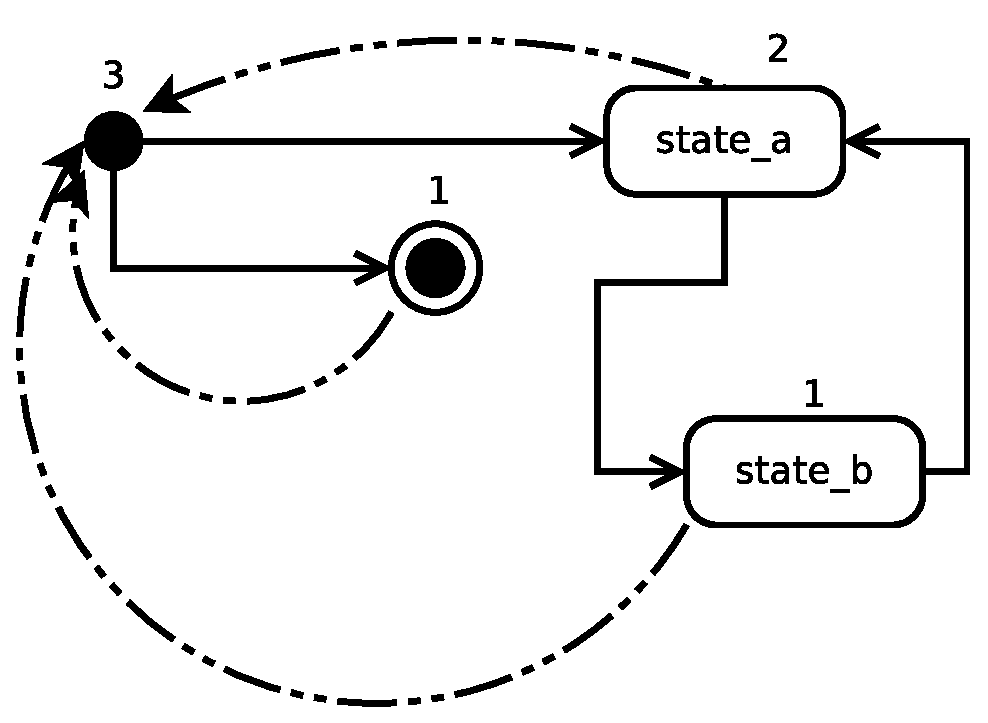
\includegraphics[width=0.6\textwidth,keepaspectratio]{img/smrefs}
  \caption{Non-transition references to the initial state. The states have the number of references over them.}
  \label{fig:smrefs}
\end{figure}
There is a case in which this recursive remove action is not enough. When we have a cycle in the graph that represents the state machine,
like the one that begins on \texttt{state\_a} in \emph{figure \ref{fig:smrefs}}, and we try to remove a transition before it, we will 
create
two non-connex graph components. This graph will be composed by a subgraph with the states from the initial to the leaving state of the 
transition we 
removed, and another from the cycle to the end. \emph{Figure \ref{fig:bism}} is the result of removing the transition from the initial
state to \texttt{state\_a}. It shows clearly the resulting graph with two non-connex components.\\
\begin{figure}[h]
  \centering
  \includegraphics[width=0.6\textwidth,keepaspectratio]{img/bism}
  \caption{Graph with two non-connex components result of removing the transition from initial state to \texttt{state\_a}.}
  \label{fig:bism}
\end{figure}
To solve this, every time we remove a transition and the destination state is not removed, we check with the BFS algorithm if there is a
path between the initial state and the destination state. If there is not, then we have found a cycle and we have to remove the whole 
subgraph.\\
\\
The {\bf event handler} is the function that deals with the received events. When talking about the adding-transition handler we mentioned
that the events from the transitions are stored in a hash table for quick access. Every time we receive an event we look in this hash table
searching by its identifier. If it didn't find anything is because the event was not expected. Otherwise if we find an event in the hash
table it means that this event is a requirement for at least one of all the transitions we have, but is not necessarily needed now.
The event from the hash table contains references to the transitions that require it in order to forward to the next state. For every
referenced transition the user that sent the event has credentials to, it adds a noticed event and when all the required events are 
noticed then it can run the action.\\
In order to run the action first we must check the kind of action the transition has assigned and then run its assigned launched according
to the data it contains.\\
If the kind of the action is \emph{NONE} it won't run any action launcher.\\
The \emph{CMD} kind of action launcher will execute the stated command in a local shell with the permissions of the owner of the state 
machine.\\
For the \emph{PROP} kind of action, the launcher will connect to the remote host, negotiate the configuration of the data transmission
discussed in \emph{section \ref{sec:users}}, and send all the events. The host will decide the credentials of the received events by
configuration and linking of users to TLS certificates.\\
Once the action has been executed it has to remove from the hash of events all the transitions that leave from the same state than the
one it executed, because from now on these events are not expected by those transitions. We forwarded to the next state. This is probably 
the most ugly and costly part of the code we have. We go through all the transitions from the same state,
which are in a list, get the events and search and dereference the current transitions. It is not hard to see that with a big number of 
transitions and events this could be a bottleneck.\\
If the action has not been executed yet, the clearing of the references to the current transitions is easier, because we only have to go to
the received event and clear it, we don't have to take into account other events that are not being expected by other transitions.\\
The last step to perform is to reference the new current transitions to its events. This is done by exploring all the events
of all the leaving transitions of the current state.
\subsection{Conceptual model}
\label{sec:dcm}
In this section we will explore all the concepts from \emph{reactord} we already explained from the abstract perspective that classes 
offer. \emph{Figure \ref{fig:cmodel}} shows the UML conceptual mode of the daemon and we can see its relations. Probably you can 
recognize most of them by the previous explanations of the functions of \emph{reactord}.\\
\label{sec:concept}
\begin{figure}[h]
  \centering
  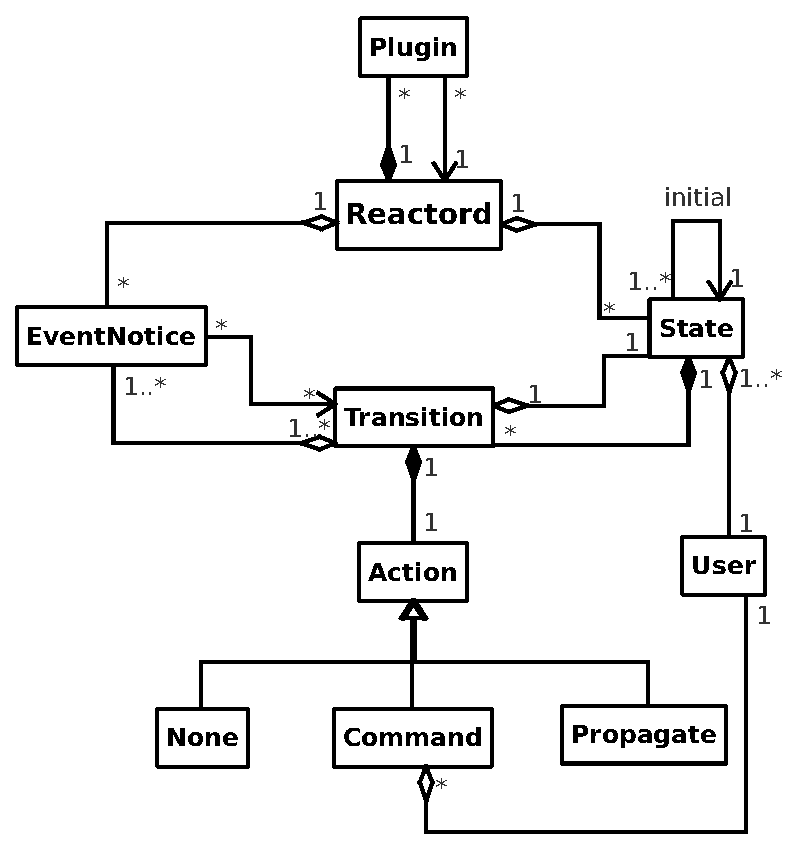
\includegraphics[width=0.75\textwidth,keepaspectratio]{img/conceptualmodel}
  \caption{\emph{reactord} UML conceptual model}
  \label{fig:cmodel}
\end{figure}
We explain every class stating the main attributes and methods, but ignoring irrelevant functions for the design like getters, setters,
constructors and destructors.
\subsubsection{Reactord}
This is the main class. Here we have the biggest part of the functionalities of \emph{reactord} and is the piece of code that the will
communicate most directly to. It contains the hash tables of events and states using their own identifier as keys for fast searching, and
the plugins loaded.
It also has the communication structures for both local control messaging and remote events receiving. These structures will be covered
with more detail in \emph{section \ref{sec:impdaemon}}.\\
\begin{list}{-}{The attributes are:}
  \item {\bf events}\\
    \texttt{Event}. Expected events in the state machines. Needed to notice them.
  \item {\bf states}\\
    \texttt{State}. This is what we use to edit the state machines. Here we have all the states with their transitions.
  \item {\bf plugins}\\
    \texttt{Plugin}. \emph{reactord} plugins loaded during the initialization.
\end{list}
\
\begin{list}{-}{The functionalities in this class are:}
  \item {\bf Daemon initialization}\\
    The daemon needs some initial checks before it starts. It is in charge of loading locating and loading the rule files, so here is where
    \emph{reactord} look for the members of the \texttt{events} user group. Also it loads the plugins from the default directory. There are
    more initializations done in here but they are more related to the implementation than to the design, so we won't cover them here.\\
    The functions are:
    \subitem \texttt{load\_users}:
      Given a group name it returns all the members of this group in a list.
    \subitem \texttt{init\_rules}:
      When called, \emph{reactord} contains the state machines from all the privileged users rule files.
    \subitem \texttt{load\_all\_modules}:
      Given a directory it loads all the valid modules located in there.
    \subitem \texttt{load\_module}:
      Given a module path, it checks if it is valid and loads it.
  \item {\bf Final rule parsing}\\
    The functions that ask for the preliminary parsing of the rules to \emph{libreactor} and make the final parsing of the action in the
    received parse tree. It is called in the daemon initialization and the result parse tree is a parameter for the state machines 
    machines management functions.\\
    The functions are:
    \subitem \texttt{parse\_rule}:
      Receives a rule string as a parameter and returns a parse tree. If there were syntax errors they must be stated on the parse tree.
    \subitem \texttt{parse\_file}:
      Receives file path string as a parameter and returns a ordered list of parse trees with the same conditions for each parse tree than
      with the \texttt{parse\_rule} function.
  \item {\bf Local control messaging management}\\
    This is only one function which for a local control message it selects de correct handler.
    \subitem \texttt{attend\_cntrl\_msg}:
      Given a communication structure (socket) with data ready to be read, it gets the message with \emph{libreactor} functions process
      it if needed and calls the correct handler. If there was any error, it sends an error message to the sender and returns an error
      code.
  \item {\bf Remote events management}\\
    \subitem As \emph{libreactor} only contains the functions to communicate with local processes, we needed actions to make the same
      but through TCP/IP. These functions are wrappers of the local control ones to make them able to connect to remote hosts. The 
      functions are:
      \subitem \texttt{listen\_remote}:
	It makes \emph{reactord} able to receive remote events. The return value is the structure for communication (socket).
      \subitem \texttt{connect\_remote}:
	It returns a structure for communication (socket) for the client to send events to a remote host.
      \subitem \texttt{receive\_remote\_events}:
	Given a communication structure (socket) with data ready to be read it returns a list of events received. For every event received
	an \texttt{ACK} message will be sent.
      \subitem \texttt{send\_remote\_events}:
	Given a communication structure (socket) connected with the server and a list of events, it sends the events one by one and
	waiting for the \texttt{ACK}. When all the events are sent it sends a final \texttt{EOM} message.
      \subitem \texttt{attend\_remote\_events}:
	Given a communication structure (socket) with data ready to be read, it gets the message and sends it to the event-noticing 
	handler. If there was any error, it sends an error message to the sender and returns an error code.\\
      \\
      Except for the \texttt{attend\_remote\_events} function, all the other functions could be in the \emph{libreactor} in the future, if 
      needed.
  \item {\bf State machines management}\\
    These functions are the operations that can be performed over the states machines. They can also be called \emph{input handlers} 
    because these operations always use input received by \emph{reactord} from external sources.
      \subitem \texttt{add\_rule\_handler}:
	Given a rule parse tree and the user credentials, it adds the transition if it is legal. If not it returns with an error code.
      \subitem \texttt{rm\_trans\_handler}:
	Given a state identifier, a transition number and the user credentials, it removes the transition and the part of the state machine
	depending on it. If there is some error occurred it returns with an error code.
      \subitem \texttt{event\_handler}:
	Given an event and the user credentials, it notices the event in its current transitions.
  \item {\bf Main loop}\\
    The main function simply enters in a loop waiting for external messages to react to. When a message is received, the correct ``attend''
    function is called. It leaves the loop when the program is stopped.
\end{list}
One could think that some of these functionalities could be isolated in different classes. For example the management functionalities
could be in a different class.\\
We put all these functionalities in the same main class because they do not use any data structure or their data structures depend on 
\emph{libreactor}. Also, as you can see \emph{Implementation section (\ref{sec:imp})}, we did not use a object oriented programming 
language, so class abstraction is not really critical for our project.

\subsubsection{State}
State is one of four principal components of the state machines, together with EventNotice, Transition and Action. It is the container and 
link between transitions and is the one that permits our software react different in different situations.\\
\begin{list}{-}{The attributes are:}
  \item {\bf id}\\
    \texttt{String}. Unique identifier of the state. It is defined by the user using rules.
  \item {\bf transitions}\\
    \texttt{Transition}. List of transitions leaving the state.
  \item {\bf fsminitial}\\
    \texttt{State}. Is a reference to the initial, and it is used as an identifier of the state machine.
  \item {\bf refcount}\\
    \texttt{Integer}. References to the state, by other states that have it as initial state or by transitions.
\end{list}
The functionalities in this class are only getters, setters, a constructor and an dereference based destructor. The cost of setting a new 
initial state to an state machine is high, because we have to go through all the states of the state machine using a BFS and changing the
\texttt{fsminitial} attribute.
\subsubsection{EventNotice}
An EventNotice is a class that represents the expectation of an event by a transition in order to go to the destination state. When we 
receive an event, we use its identifier to find its EventNotice and obtain the transitions they are related to.\\
\begin{list}{-}{The attributes are:}
  \item {\bf id}\\
    \texttt{String}. Unique identifier of the event we expect to notice. It is defined in the rules.
  \item {\bf currtrans}\\
    \texttt{Transition}. List of the transitions that are leaving the current states of all the state machines and have the EventNotice as 
    a requirement for its advance.
  \item {\bf refcount}\\
    \texttt{Integer}. References to the EventNotice by transitions that require it.
\end{list}
The functionalities in this class are only getters, setters, a constructor and an dereference based destructor. 
\subsubsection{Transition}
It is the backbone of the whole project. It binds the other state machine classes together and contains the reacting conditions and the
reaction in the same class.\\
\begin{list}{-}{The attributes are:}
  \item {\bf enrequisites}\\
    \texttt{EventNotice}. It is a list of EventNotices required to advance in the state machine by this transition.
  \item {\bf eventnotices}\\
    \texttt{Integer}. It is a counter of EventNotices.
  \item {\bf noticedevents}\\
    \texttt{Integer}. It is a counter of events already noticed. When this counter equals \texttt{eventnotices}, then we can advance and 
    launch the action.
  \item {\bf destination}\\
    \texttt{State}. \texttt{destination} is a reference to the destination State of the transition.
  \item {\bf action}\\
    Reference to the action to be launched when all the required events are noticed.
\end{list}
It has several getters and setters, but the most important function of this class is:
\begin{list}{}{}
  \item \texttt{notice\_event}:
    This function adds one to the \texttt{noticedevents} counter. If this counter equals \texttt{eventnotices} then it can launch the
    action and return \texttt{true}. If not it returns \texttt{false}.
\end{list}
\subsubsection{Action}
What we have to do when the transition is executed. As we can see and we already said in the model it can be of three kinds. NONE, CMD and
PROP.\\
Action by itself does not have important attributes but it has an important method:
\begin{list}{}{}
  \item \texttt{action\_do}:
    It checks the kind of action it is dealing with and calls the correct action launcher. In case of NONE Action, no launcher is called.
\end{list}
\begin{itemize}
  \item {\bf NONE}\\
    It has neither attributes nor methods. It is used when the user only wants to advance to the next State.
  \item {\bf CMD}\\
    This kind of Action runs shell commands.
    \begin{list}{-}{The attributes are:}
      \item {\bf user}\\
	\texttt{User}. User privileges that will be used to run the command.
      \item {\bf cmd}\\
	\texttt{String}. Command to run in the shell.
    \end{list}
    \
    \begin{list}{}{And the methods:}
      \item \texttt{cmd\_execute}:
	It is the command launcher. It runs the command in a shell.
    \end{list}
  \item {\bf PROP}\\
    This kind of Action propagates all the events received by the Transitions at the same time.
    \begin{list}{-}{The attributes are:}
      \item {\bf addr}\\
	\texttt{String}. Host IP address or address name in a string.
      \item {\bf port}\\
	\texttt{String}. Integer defining the port.
      \item {\bf enids}\\
	\texttt{String}. List of events identifiers to propagate.
    \end{list}
    \
    \begin{list}{}{And the methods:}
      \item \texttt{prop\_execute}:
	Propagates the events to the remote host.
    \end{list}
\end{itemize}

\subsubsection{User}
This class contains the information about a user, so \emph{reactord} can load the 'events' group users rule files and control the 
credentials. As we already know we are going to use UNIX as our software platform, we can say that the attributes of the class will be 
simply the \texttt{passwd} struct offered by POSIX implementations\cite{og:pwdh}:
\begin{list}{-}{}
  \item {\bf pw\_name}\\
    \texttt{String}. User's login name.
  \item {\bf pw\_uid}\\
    \texttt{Integer}. Numerical user ID.
  \item {\bf pw\_gid}\\
    \texttt{Integer}. Numerical group ID. 
  \item {\bf pw\_dir}\\
    \texttt{String}. Initial working directory.
  \item {\bf pw\_shell}\\
    \texttt{String}. Program to use as shell.
\end{list}
There are no methods instead of constructor and destructor.
\subsubsection{Plugin}
Here \emph{reactord} manages the information about the loaded plugins. This information is retrieved by the plugin itself when it is
loaded to the daemon.
\begin{list}{-}{The attributes are:}
  \item {\bf modhandler}\\
    \texttt{Integer}. Reference to the loaded module handler.
  \item {\bf name}\\
    \texttt{String}. The name of the plugin. It must be unique.
  \item {\bf version}\\
    \texttt{Integer}. Version of the plugin named \texttt{name}. It can be useful for managing different versions of the same plugin.
  \item {\bf pt}\\
    \texttt{Integer}. This is a reference to the \texttt{pthread} running the job-scheduler or event trigger worker.
\end{list}
~
\begin{list}{-}{By now, the methods are:}
  \item \texttt{init}:
    This is the function that returns the set of function callbacks available in the plugin and information like the name and version.
  \item \texttt{start\_worker}:
    This is the thread main function for the job-scheduler worker.
  \item \texttt{stop\_worker}:
    It stops the the thread main function.
\end{list}
\section{Command line program}
This is a really little program called \emph{reactorctl}. Its purpose is the communication between the user and the daemon. It is so 
simple that it is not even needed to show a conceptual model, because it uses \emph{libreactor} to perform all the communication with the 
daemon.\\
It only has a main function that checks the input arguments of the program.
\begin{itemize}
  \item \texttt{-e}: \emph{Send an event to the daemon}. This argument is followed by an event identifier to send to the local 
    \emph{reactord}. When sent it is expected to receive an \texttt{ACK} message in response. If another kind of message or none is 
    received, then it informs the user about an error in the communication.
  \item \texttt{-a}: \emph{Add a rule}. It is followed by a rule using the syntax defined in \emph{section \ref{sec:rparser}}. There is no
    processing of this string in the \emph{reactord} side, it simply sends it to the \emph{reactorctl} and waits for an informational
    response. The expected messages are:
    \subitem \texttt{ACK} - Everything went fine.
    \subitem \texttt{ARG\_MALFORMED} - There was a syntax error. It is logged using the system logger.\\
    If another kind of message or none is received, then it informs the user about an error in the communication.
  \item \texttt{-r}: \emph{Remove a transition}. It is followed by a transition identifier formed by a transition leaving state identifier
    and the number of leaving transition, separated by a dot. i.e.: ``\texttt{STATE\_A.1}''. There is no processing of this string in the 
    \emph{reactord} side, it simply sends it to the \emph{reactorctl} and waits for an informational response. The expected messages are:
    \subitem \texttt{ACK} - Everything went fine.
    \subitem \texttt{ARG\_MALFORMED} - The string is not of the form ``string.number''.
    \subitem \texttt{NO\_TRANS} - The transition defined by the pseudo-identifier does not exist.\\
    \\
    If another kind of message or none is received, then it informs the user about an error in the communication.
\end{itemize}

\section{Shared library}
\label{sec:lib}
In this component of \emph{reactor} is where we put every piece of code that we think that would be useful for developers that want to
extend its functionalities, or make use of the existing ones in their applications.
\begin{list}{-}{So we could divide its main use cases in two:}
  \item \emph{reactord} plugins.
  \item External programs.
\end{list}
Now we are going to discuss the design of the different parts in which the shared library is divided, and explain the expected uses of them.
\subsection{Control}
\label{sec:cntrl}
This component of the shared library is in charge of the communication of control messages between a server (\emph{reactord}) and a local
client, for example \emph{reactorctl}. The messages are obviously divided by requests by the client and responses by the server.\\
This component of \emph{libreactor} is specially not expected to be used \emph{reactord} plugins because it does not make sense. The
biggest advantage of the plugin system is that the communication is at function level, so this is not needed.
\begin{list}{-}{It mainly has to:}
  \item Make the caller listen for peers.
  \item Connect to a listening peer.
  \item Send a message in the correct format to the listening peer.
  \item Read a received message.
  \item Stop the caller from listening peers.
\end{list}
\subsubsection{Wire protocol}
\label{sec:wire}
The communication is performed through a simple wire protocol\cite{pcm:wire}, based on two initial integers in the message defining the 
its size and its mutually known kind of message. \emph{Figure \ref{fig:wire}} shows an scheme of the structure of a message.
\begin{figure}[t]
  \centering
  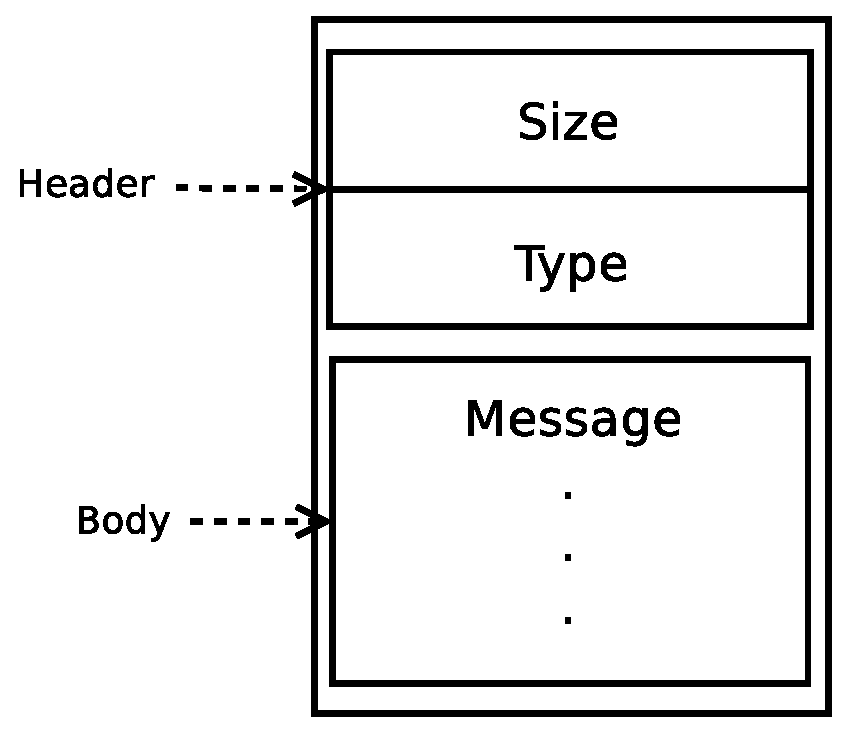
\includegraphics[width=0.5\textwidth,keepaspectratio]{img/wire}
  \caption{\emph{reactor} wire protocol message structure.}
  \label{fig:wire}
\end{figure}
As we can see the {\bf header} of the message only contains two fields:
\begin{itemize}
  \item \texttt{Size}: This is the size of the message's body in bytes. It is limited by the size of the strings in the operating
    system, and the size of the field is the size of an integer in the operating system.
  \item \texttt{Type}: It is an integer that identifies the contents of the message's body. The possible types of message are:
    \subitem \texttt{EVENT} - The body message is an string with the identifier of an event. This type of message is sent by the client
      as a request.
    \subitem \texttt{ADD\_RULE} - The body of the message is an string with a rule with the format defined in \emph{section 
      \ref{sec:rparser}}. This type of message is sent by the client as a request.
    \subitem \texttt{RM\_TRANS} - The body of the message is an string with a transition pseudo-identifier. The format is a leaving state 
      identifier and the number of transition. i.e.: ``STATE\_A.1''. This type of message is send by the client as a request.
    \subitem \texttt{EOM} - This type of message is used to mark the end of a sequence of messages. i.e. a list of events. 
      This type of message is send by the client as the end of a request.
    \subitem \texttt{ACK} - It confirms that the actions requested by the client were performed as expected. It doesn't have body 
      message. This type of message is send by the server as a response.
    \subitem \texttt{RULE\_MULTINIT} - As response of an \texttt{ADD\_RULE} message, it states that the rule is illegal because tries to 
      create a state machine with several initial states. It doesn't have body message. This type of message is send by the server as a 
      response.
    \subitem \texttt{ARG\_MALFORMED} - The request to which this message is response to is malformed. It doesn't have body message. 
      This type of message is send by the server as a response.
    \subitem \texttt{NO\_TRANS} - As a response of a \texttt{RM\_TRANS} message, it states that the transition defined by its 
      pseudo-identifier does not exist. It doesn't have body message. This type of message is send by the server as a response.
\end{itemize}
The message {\bf body} only contains one field defined by the protocol:
\begin{itemize}
  \item \texttt{Message}: Here is were the contents of the message are. The format is not defined by the protocol itself, but by the
    \texttt{Type} field.
\end{itemize}
\subsubsection{Conceptual model}
\emph{Figure \ref{fig:controlcm}} shows the conceptual model of the \emph{libreactor}'s control component. \texttt{Message}, 
\texttt{Header} and \texttt{Body} have their attributes are the same as the message fields explained in \emph{section \ref{sec:wire}}.
\begin{figure}[h]
  \centering
  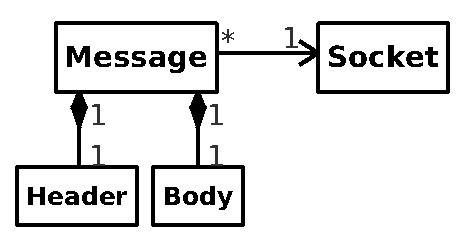
\includegraphics[width=0.5\textwidth,keepaspectratio]{img/controlcm}
  \caption{Conceptual model of the \emph{libreactor}'s control component.}
  \label{fig:controlcm}
\end{figure}
\begin{list}{}{}
  \item {\bf Message}\\
    \\
    The attributes are the same as the message fields explained in \emph{section \ref{sec:wire}}.
    \subitem Functions:
      \subsubitem \texttt{send}:
	It sends the message using the \texttt{Socket} and waits for the response from the peer. If the response is \texttt{ACK} returns
	0, but if it is different or nonexistent it will return an error code.
      \subsubitem \texttt{receive}:
	It receives a message using the \texttt{Socket} and the wire protocol.
  \item {\bf Header}\\
    \\
    The attributes are the same as the message fields explained in \emph{section \ref{sec:wire}} and it has no methods beyond getters and
    setters.
  \item {\bf Body}\\
    \\
    The attributes are the same as the message fields explained in \emph{section \ref{sec:wire}} and it has no methods beyond getters and
    setters.
  \item {\bf Socket}\\
    \\
    Bridge for the communication with the peer.
    \subitem Attributes:
      \subsubitem {\bf sfd} \\
	\texttt{Integer}. Reference to the operating system internal data structure to perform communication between programs.
    \subitem Functions:
      \subsubitem \texttt{listen}:
	Constructor. It returns a listening server socket.
      \subsubitem \texttt{connect}:
	Constructor. It connects to the local \emph{reactord} socket, and returns the client socket for the connection.	
\end{list}
\subsection{Parser}
\label{sec:parser}
The \emph{libreactor}'s parser generates parse trees from strings and simple grammar definitions. It is expected to be used in the 
\emph{reactord} plugins development.
\subsubsection{Grammar definition}
This is an almost-generic parser. It means that it doesn't parse only one grammar, but several of them thanks to a previous 
configuration. This is possible because we think we only need quiet simple grammars that define unrelated expressions that can contain
listed and nested inner expressions, but at least by now, we don't care about how the final tokens may look.\\
What defines an expression and configures the grammar are five parameters:
\begin{itemize}
  \item {\bf Subexpression separator} - Character used to separate subexpressions in the parent expression.
  \item {\bf End mark} - Character used to mark the end of the expression.
  \item {\bf Trim} - If used, it removes the useless initial and ending of an expression.
  \item {\bf Subexpression number} - The number of the subexpression those parameters define in the parent expression.
  \item {\bf Subexpressions} - Parameters for the inner expressions.
\end{itemize}
Also, this parser allows comments. Everything after a \texttt{\#} character will be ignored by the parser.\\
As this is part of a shared library , let's take as example a crontab, instead of one of our use cases. We have seen before this 
crontab entry:
\begin{center}
  \texttt{1 0 {*} {*} {*}  reactorctl -e cron\_event\_1}\\
\end{center}
This crontab entry means that every day at \texttt{00:01} it will execute the command \texttt{reactorctl -e cron\_event\_1}. In 
\emph{table \ref{tab:crontab}} we can see the meaning of the fields and the allowed values. Obviously, the last field is the command to
execute.
\begin{table}[h]
  \begin{center}
    \begin{tabular}{| c | c | c | }
      \hline
      {\bf Field name} & {\bf Allowed values} & {\bf Allowed special characters} \\ \hline
      Minutes & 0-59 & * / , - \\ \hline
      Hours & 0-23 & * / , - \\ \hline
      Day of month & 1-31 & * / , - ? L W \\ \hline
      Month & 1-12 or JAN-DEC & * / , - \\ \hline
      Day of month & 0-6 or SUN-SAT & * / , - ? L \# \\ \hline
    \end{tabular}
    \caption{Format of a crontab sorted by fields appearance.}
    \label{tab:crontab}
  \end{center}
\end{table}
Our parser, as we said, does not care about the allowed values. This must be checked lately. But we can see clearly three rules for the
generation of a parse tree that our parser can use.\\
First of all, the whole expression is a line, so the end mark is the \texttt{EOL} character.\\
Also we can see that, except for the last field, all the fields are separated by the white space character. We also have to take into
account that if between field we have several white spaces, it doesn't mean that we have empty values, so we should trim it.
Finally the rule always have six fields, so the sixth field is the last one no matter what it contains.\\
The resulting configuration would be:
\begin{list}{-}{}
  \item {\bf Subexpression separator}: ' '
  \item {\bf End mark}: \texttt{EOL}
  \item {\bf Trim}: Yes
  \item {\bf Subexpression number}: -
  \item {\bf Subexpressions}:
    \subitem {\bf Subexpression separator}: \texttt{EOL}
    \subitem {\bf End mark}: \texttt{EOL}
    \subitem {\bf Trim}: No
    \subitem {\bf Subexpression number}: 6
    \subitem {\bf Subexpressions}: None
\end{list}
Using the end mark character as subexpression separator is the way to say that there is no separator.
\subsubsection{Result}
The result of the parsing process is a structure as it is defined by grammar definition. If the expression had a wrong syntax, then
the result should inform about the error instead.\\
The structure is a simple tree with the main exception at the root, the subexpressions as branches and the tokens as leaves. 
\begin{list}{-}{Our example's result would look like this:}
  \item {\bf Expression}:
    \subitem {\bf Subexpression 1}: 1
    \subitem {\bf Subexpression 2}: 0
    \subitem {\bf Subexpression 3}: *
    \subitem {\bf Subexpression 4}: *
    \subitem {\bf Subexpression 5}: *
    \subitem {\bf Subexpression 6}:
      \subsubitem {\bf Subexpression 1}: reactorctl -e cron\_event\_1
\end{list}
\subsubsection{Conceptual model}
\begin{figure}[h]
  \centering
  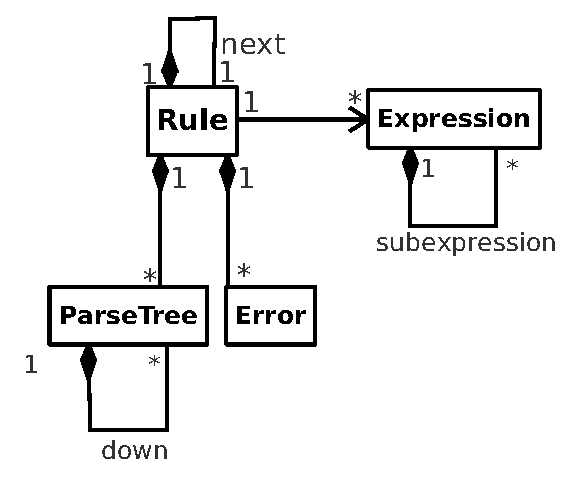
\includegraphics[width=0.65\textwidth,keepaspectratio]{img/parsercm}
  \caption{Conceptual model of the \emph{libreactor}'s parser component.}
  \label{fig:parsercm}
\end{figure}
\begin{list}{}{}
  \item {\bf Rule}\\
    \\
    The main class of the parser, contains the parse tree and the information related.
    \subitem Attributes:
      \subsubitem {\bf line}\\
	\texttt{String}. The unparsed rule.
      \subsubitem {\bf expr}\\
	\texttt{Expression}. The definition of the grammar.
      \subsubitem {\bf linen}\\
	\texttt{Integer}. Number of line of the rules file. -1 if the rule was not extracted from a file.
      \subsubitem {\bf file}\\
	\texttt{String}. Path to the rules file. Empty if the rule was not extracted from a file.
      \subsubitem {\bf ptree}\\
	\texttt{ParseTree}. Result parse tree from the \texttt{linen}. If \texttt{errors} is not empty, \texttt{ptree} is.
      \subsubitem {\bf errors}\\
	\texttt{Error}. If in the parse process any error was detected it is specified here. If \texttt{ptree} is not empty, 
	\texttt{errors} is.
      \subsubitem {\bf next}\\
	\texttt{Rule}. Next rule in the same file.
    \subitem Functions:
      \subsubitem \texttt{parse\_rule}:
	Parses \texttt{line}.
      \subsubitem \texttt{parse\_file}:
	Parses all the lines in \texttt{file}.
  \item {\bf Expression}\\
    \\
    The simple grammar definition.
    \subitem Attributes:
      \subsubitem {\bf exprnum}\\
	\texttt{Integer}. Is the number of subexpression from its parent which grammar this \emph{Expression} class defines. If it defines
	the root expression this value is not needed.
      \subsubitem {\bf tokensep}\\
	\texttt{Character}. Subexpressions separator character.
      \subsubitem {\bf end}\\
	\texttt{Character}. Expression end mark character.
      \subsubitem {\bf trim}\\
	\texttt{Boolean}. If true, ignore all the white spaces at the beginning and at the end of the subexpressions when parsing.
      \subsubitem {\bf subexpr}\\
	\texttt{Expression}. List of \texttt{Expressions} sorted by order of appearance.\\
      \\
      The functions are only getters, setters, constructor and destructor.
  \item {\bf Error}\\
    \\
    Rule malformed syntax information.
    \subitem Attributes:
      \subsubitem {\bf pos}\\
	\texttt{Integer}. Position where the beginning of the error is located.
      \subsubitem {\bf msg}\\
	\texttt{String}. Message with information about the error.\\
    \\
    The functions are only getters, setters, constructor and destructor.
  \item {\bf ParseTree}\\
    \\
    The result of a correct rule parsing.
    \subitem Attributes:
      \subsubitem {\bf data}\\
	\texttt{String}. It is the content of this token.
      \subsubitem {\bf down}\\
	\texttt{ParseTree}. List of subexpressions.
      \subsubitem {\bf pos}\\
	\texttt{Integer}. Position in the unparsed rule string.\\
    \\
    The functions are only getters, setters, constructor and destructor.
\end{list}
\subsection{Plugins interface}
\label{sec:plugins}
Here we have data structures and the definition of functions needed both by \emph{reactord} and the plugins. It does not contain 
any implementation, so we won't show any conceptual model here. In the other hand we will explain the data structures and function 
definition from both sides.\\
\subsubsection{Data structures}
We only have three shared data structures.\\
\\
\begin{list}{-}{PluginInfo}
  \item {\bf version}\\
    \texttt{Version}. Version of the plugin.
  \item {\bf name}\\
    \texttt{String}. Name of the plugin.
\end{list}
\begin{list}{-}{PluginServices}
  \item {\bf version}\\
    \texttt{Version}. Version of the plugin manager.
\end{list}
\begin{list}{-}{Version}
  \item {\bf major}\\
    \texttt{Integer}. Major version number.
  \item {\bf minor}\\
    \texttt{Integer}. Minor version number.
\end{list}
\subsubsection{Function definitions}
We will divide this by two groups of functions.
\begin{itemize}
 \item Implemented by \emph{reactord}:
  \subitem \texttt{Event handler}: Given a an event identifier, the function notices it.
 \item Implemented by the plugins:
  \subitem \texttt{init\_plugin}: Given a \texttt{PluginServices} it returns the plugin's \texttt{PluginInfo}.
  \subitem \texttt{main\_thread}: It is called as a thread and it executes the plugin's job scheduler.
\end{itemize}
\subsection{Data log}
\label{sec:log}
This part of \emph{libreactor} for storing log messages. By now it is a simple wrapper to the \emph{syslog} API\cite{man:syslog}.
\begin{list}{-}{We consider four levels of messages:}
  \item \texttt{INFO}: An informational message. It only informs about something the software did in a normal workflow.
  \item \texttt{WARNING}: It is an alert about something unexpected that can lead to future malfunctions of the software.
  \item \texttt{ERROR}: Something went wrong and the software failed.
  \item \texttt{DEBUG}: Like \texttt{INFO}, but it is information only useful when debugging the software.
\end{list}
In order to do that \emph{libreactor} offers a set of log functions:
\begin{list}{-}{}
  \item \texttt{info}: Given a string this function logs it as an \texttt{INFO} message.
  \item \texttt{warn}: Given a string this function logs it as an \texttt{WARNING} message.
  \item \texttt{err}: Given a string this function logs it as an \texttt{ERROR} message. 
  \item \texttt{dbg}: Given a string this function logs it as an \texttt{DEBUG} message, only if the program is in debug mode.
  \item \texttt{dbg\_e}: Given a string this function logs it as an \texttt{WARNING} message with the errno value, only if the program
    is in debug mode.
  \item \texttt{die}: Given a string this function logs it as an \texttt{ERROR} message and exits the program.
  \item \texttt{close\_log}: Closes the connection with \emph{syslog} if any.
\end{list}

% \section{Plugins}
% TODO Extend report contents